\begin{figure}[t]
\begin{center}
	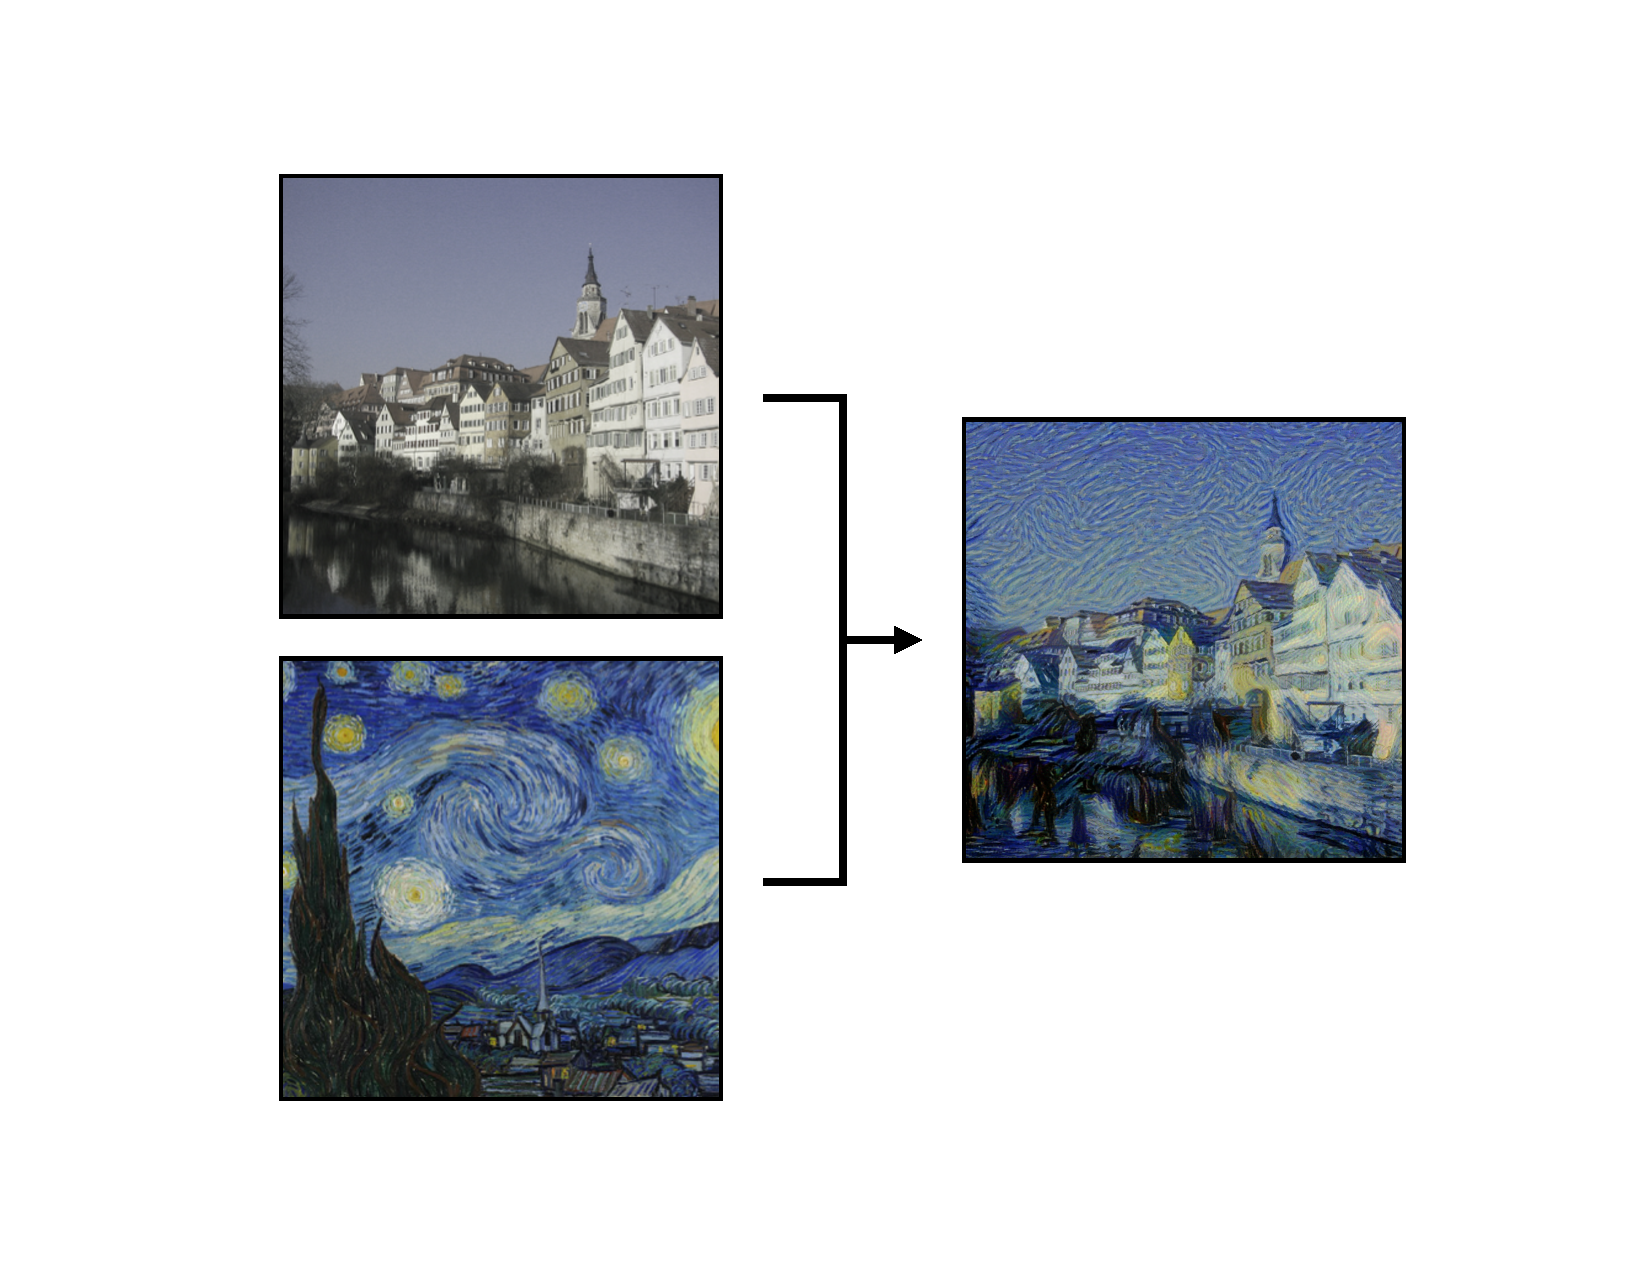
\epsfig{file=style_transfer.pdf, width = 0.6\textwidth}\\
	\caption[Image style transfer]{Image style transfer. The goal is to synthesize a texture (right) from a source image (bottom-left) while constraining the process in order to preserve the semantic content of another image (top-left).}
	\vspace{-0.65cm}
	\label{fig:style_transfer}
\end{center}
\end{figure}